\section{Produktbeschreibung und Funktion}

Aufgrund der Resultate der Evaluation der Lösungsprinzipien wurde beschlossen, 
das Konzept der stationären Abschussvorrichtung (Drehturm) weiter 
auszuarbeiten. 

Hierbei handelt es sich um ein nicht fahrbares, autonom arbeitendes Gerät mit 
einer in horizontaler Richtung drehbaren Abschussvorrichtung. Der gesamte Aufbau 
des Abschussmechanismus inklusive Balllager befindet sich auf einer drehbaren 
Plattform, welche auf einem geeignetem Stativ platziert ist. Die Plattform 
wird durch einen Schrittmotor und eine Zahnradübersetzung präzise in Position 
gebracht. Der Abschusswinkel in vertikaler Richtung ist hierbei fixiert. 

Die Abschussvorrichtung besteht im wesentlichen aus einem Balllager, einer 
Ballnachführung und einem sich schnell drehenden Rad, welches die Bälle auf 
die gewünschte Abschussgeschwindigkeit beschleunigt. Die Bauweise dieser drei 
Komponenten soll integral erfolgen, wobei das längliche, Quaderförmige 
Balllager als Hauptstruktur dient. An diesem sind sowohl das Rad für die 
Ballbeschleunigung als auch die Komponenten der Ballnachführung befestigt.

\subsection{Drehvorrichtung}
Das unterste Element des Gerätes besteht aus einer kleinen, möglichst leichten 
Bodenplatte. An dieser Bodenplatte werden drei Beine (Rohrform) angeschraubt. Mit 
zwei Axial-Kugellagern wird ein grosses Zahnrad (z1=120) auf der Bodenplatte 
befestigt. Auf dieses wird anschliessend der gesamte Aufbau bestehend aus Turm, Balllagerung und Abschussvorrichtung montiert. 

\begin{figure}[h!]          
	\centering             
	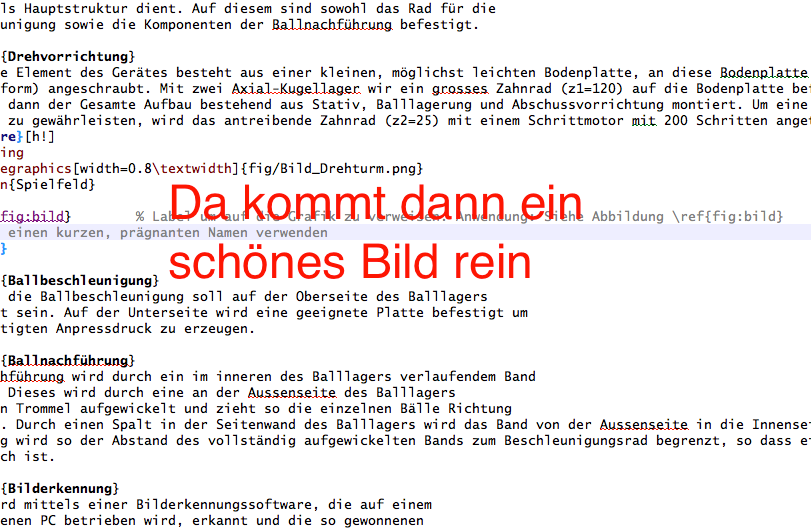
\includegraphics[width=0.8\textwidth]{fig/Bild_Drehturm.png}    
	\caption{Drehvorrichtung}
	
	\label{fig:bild}        % Label um auf die Grafik zu verweisen. Anwendung: Siehe Abbildung \ref{fig:bild}
	% Bitte einen kurzen, prägnanten Namen verwenden
\end{figure}

Um eine genaue Ausrichtung zu gewährleisten, wird das antreibende Zahnrad 
(z2=25) mit einem Schrittmotor mit 200 Schritten angetrieben (QSH 4218, 
QMot.eu). Bei 200 Schritten ergibt sich eine Genauigkeit von 1.8$^\circ$, mit einer 
Übersetzung von z1/z2=4.8 ergibt das eine Ausrichtgenauigkeit von 0.375$^\circ$. Dies 
bedeutet für eine Distanz von 1900mm eine seitliche Abweichung von 
$1900 \cdot \tan(0.375^\circ)= 12.5mm$. Somit wird diese Abweichung bei einem 
Korbdurchmessen von 30cm keine Rolle spielen. Des weiteren wird mit einem 
geeigneten Treiber sogar noch eine höhere Genauigkeit erreicht 
(Zwischenschritte), welche jedoch vom Drehmoment abhängig ist. 

\subsection{Ballbeschleunigung}
Das Rad für die Ballbeschleunigung soll auf der Oberseite des Balllagers 
positioniert sein. Auf der Unterseite wird eine geeignete Platte befestigt um 
so den benötigten Anpressdruck zu erzeugen. 
Die Beschleunigung des Rads soll mittels einem integrierten brushless Motor erfolgen. Hierzu wird das Rad selbst hergestellt und die benötigten Magnete direkt in der Felge verbaut. Das Grundgerüst für den Stator kann aus einem alten Motor ausgebaut und verwendet werden. Jedoch wird die Wicklung für eine angepasste Funktionalität selbst aufgebracht.

\subsection{Ballnachführung}
Die Ballnachführung wird durch ein im Inneren des Balllagers verlaufendes Band 
realisiert. Dieses wird durch eine an der Aussenseite des Balllagers 
angebrachten Trommel aufgewickelt und zieht so die einzelnen Bälle in Richtung 
Abschussrad. Durch einen Spalt in der Seitenwand des Balllagers wird das Band 
von der Aussenseite in die Innenseite geführt. Gleichzeitig wird so der 
Abstand des vollständig aufgewickelten Bands zum Beschleunigungsrad begrenzt, 
so dass ein Verklemmen nicht möglich ist.
Die Trommel wird durch einen, mit einem Zahnriemen verbundenen Schrittmotor angetrieben.

\subsection{Bilderkennung}
Ziel der Bilderkennung ist es, zu erkennen wo sich der Korb auf der Spielfläche befindet. Das Bild muss so verarbeitet werden, dass in einem ersten Schritt der Korb erkannt wird und in einem zweiten Schritt die Position errechnet werden kann.
\subsubsection{Hardware}
Bei der Bildverarbeitung ist zu beachten, dass sie sehr rechen- wie auch speicherintensiv ist. Um eine Analyse eines Bildes durchzuführen sind diverse mathematische Funktionen wie auch farb-analytische Schritte nötig. Je schneller die Berechnung ausgeführt werden soll, desto grössere Rechenleistungen werden benötigt. Deshalb wurde entschieden, die Bildverarbeitung auf ein Notebook auszulagern. Dieses sollte neben genügend Speicher auch ausreichend Rechenleistung zu Verfügung stellen können. Da sämtliche Studierende bereits über ein Notebook verfügen, vereinfacht sich die gemeinsame Entwicklung auf dem Endgerät.

\subsubsection{Software}
Als Entwicklungssprache für die Bildverarbeitung hat sich die Gruppe, basierend auf der Technologierecherche, für Java entschieden. Dies vor allem auch weil sämtliche Elektrotechnik- und Informatikstudierende aufgrund der besuchten Module bereits Erfahrungen mit Java sammeln konnten. Doch Java ist auch bezüglich der Komptabilität und Schnittstellen mit diversen Entwicklungsumgebungen und Sprachen die erste Wahl. Die vorhandenen Entwicklungsumgebungen können dank der breiten Community durch die zahlreichen Plug-ins fast beliebig erweitert werden.
Die Technologierecherche hat ergeben, dass sich OpenCV als geeignetste Bildverarbeitungsbibliothek zeigt. Dies unter anderem auch, weil es über eine sehr grosse und auch aktive Community verfügt. Ebenfalls auf Grund der grossen Beliebtheit von OpenCV werden sehr viele Plattformen unterstützt, was uns bei der Wahl unserer Betriebssystemen, Komponenten und Entwicklungsumgebungen kaum einschränkt.

\subsection{Signalübertragung}
Die Signalübertragung befasst sich mit der Kommunikation zwischen den beteiligten Komponenten. Einerseits wird ein leichtgewichtiges Signal benötigt um den Start und das Ende der Aufgabe zu symbolisieren. Für die Übertragung des Bildes ist allerdings ein Übermittlungsstandard nötig, der auf eine grössere Bandbreite zurückgreifen kann.

\begin{figure}[h!]          
	\centering             
	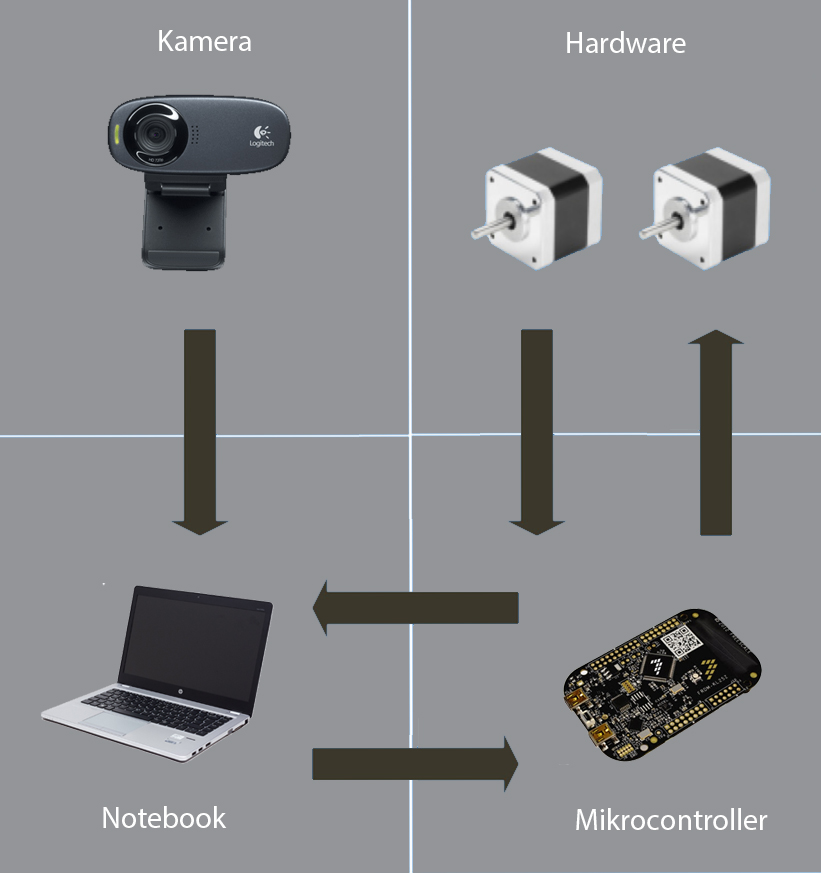
\includegraphics[width=0.5\textwidth]{fig/kommunikationsablauf.jpg}    
	\caption{Kommunikationsablauf}
	
	\label{fig:Kommunikationsablauf}
\end{figure}
\noindent
\subsubsection{Start- und Endsignal}
Das Startsignal wird drahtlos vom Laptop auf den Roboter übertragen. Nachdem dieser die Aufgabe ausgeführt hat, sendet dieser wiederum drahtlos das Endsignal an den Laptop. Aufgrund der Technologierecherche wurde entschieden, dass Bluetooth sich am Besten für diese Übertragung eignet. Nach der Erweiterung durch entsprechende Module unterstützt Bluetooth sowohl Mikrocontroller als auch reguläre Computer. Die vorgegebenen Schnittstellen vereinfachen die drahtlose Kommunikation.
\subsubsection{Befehlsübermittlung an Turm}
Für die Übertragung der Befehle an den Turm wird ebenfalls Bluetooth verwendet. Nachfolgend ist eine Liste mit möglichen Befehlen zur Steuerung des Turms und einer kurzen Beschreibung zu sehen:
\begin{itemize}
	\item \textbf{turnRight(Ticks):} Dreht den Turm die übergebene Anzahl Ticks nach rechts (negative Ticks ergeben eine Drehung nach links).
	\item \textbf{shoot:} Initiiert den Schuss.
	\item \textbf{fill:} Wird zum Zurücksetzen des Bandes verwendet.
	\item \textbf{resetTower:} Dreht den Turm wieder in die neutrale Position zurück, setzt ebenfalls das Band zurück.
	\item \textbf{statusPosition:} Erfragt die Drehstellung des Turms in Ticks (0 ist bei Endschalter).
	\item \textbf{statusBat:} Erfragt Akkuspannung (praktisch für Hinweise, ob Akku geladen werden soll oder nicht).
	\item \textbf{statusShoot:} - Erfragt aktuelle Drehzahl des Rads
	\item \textbf{statusFeed:} - Erfragt, wo die Position der Ballnachführung ist
\end{itemize}
Die Befehle werden als Strings übermittelt.
\subsubsection{Bildübermittlung}
Je höher die Auflösung des vorhandenen Bildes, desto genauer kann die Position vom Laptop bestimmt werden. Je höher die Auflösung, desto grösser wird die Bilddatei die zum Laptop übermittelt werden muss. Am naheliegendsten wäre die Verwendung von Bluetooth gewesen. Doch aufgrund von ungenügender Bandbreite muss auf einen anderen Übermittlungsstandard zurückgegriffen werden. Die Bildübertragung kann unabhängig vom Mikrocontroller geschehen. So kann sich dieser alleine auf die Abarbeitung des Schiessvorgangs konzentrieren. Das Bild wird separat entweder direkt von einer Kamera oder von einem weitere Mikrocontroller übermittelt. Um diese Übermittlung durchzuführen wurde WLAN ausgewählt. Dies vorallem, weil WLAN ein sehr verbreiteter Standard ist und fast von allen Geräten unterstützt wird. Zudem können im Handel preisgünstig WLAN-fähige Kameras erworben werden.
